\documentclass{beamer}
\usepackage{float}
\usetheme{Warsaw}
\setbeamertemplate{frame numbering}[fraction]
\title{Projectile Motion with drag}
\author{Lucky Upadhayay\and Anurag Das}
\institute{S.G.T.B. Khalsa College, University of Delhi, Delhi-110007, India}
\date{\today}
\begin{document}
\begin{frame}
    \titlepage
\end{frame}
%%%%%%%%%%%%%%%%%%%%%%%%%%%%%%%%%%%%%%
\begin{frame}[t]{Plan of talk}
    \vspace{10pt}
    Anurag Das (2020phy1116) will begin the presentation with the following sections:
    \begin{itemize}
        \item Theory
        \item Packages and methods used
    \end{itemize}
    ... and will be followed by Lucky Upadhayay (2020phy1041) taking over for the following sections:
    \begin{itemize}
        \item Results and anaylsis
        \item Conclusion
    \end{itemize}
\end{frame}
%%%%%%%%%%%%%%%%%%%%%%%%%%%%%%%%%%%%%%
\begin{frame}[t]{Theory}
    \vspace{5pt}
    \begin{block}{Projectile Motion}
    An object that is in flight after being thrown or projected is called a projectile. Such a projectile might be a football, a cricket ball, javelin or any other object.
    \end{block}
    \begin{figure}
    \centering
    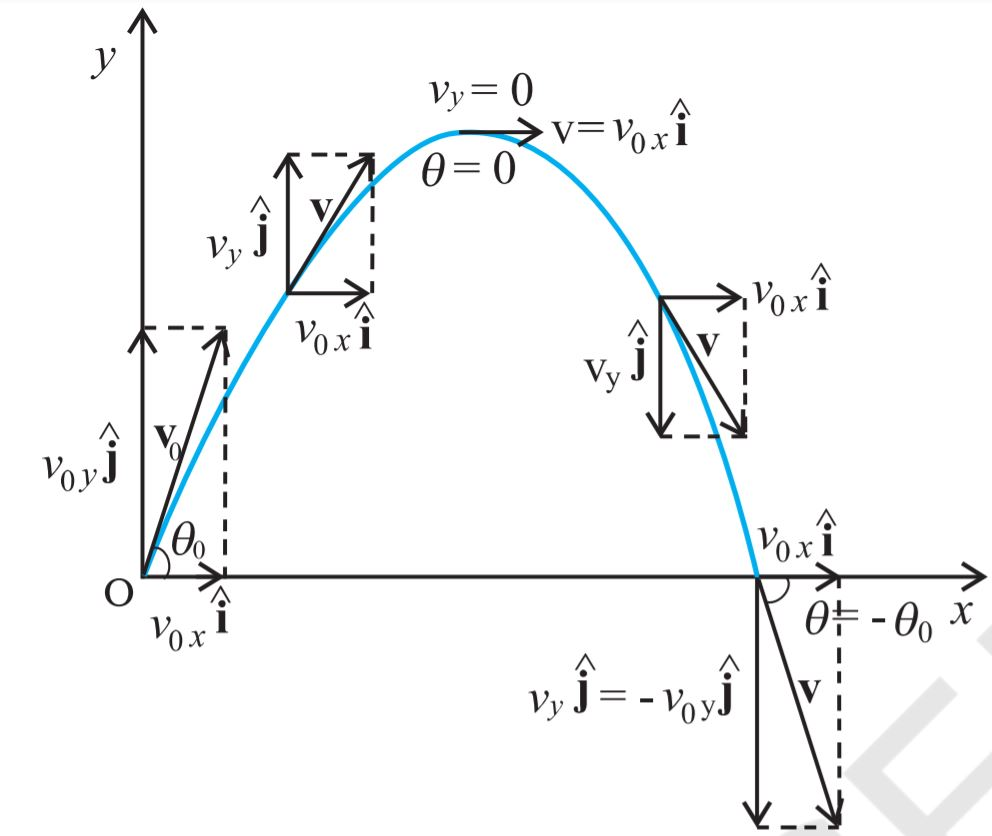
\includegraphics[width=0.45\textwidth]{fig1.JPG}
    \caption{Path of a projectile is a parabola}
    \label{fig:fig1.JPEG}
\end{figure}
\end{frame}
%%%%%%%%%%%%%%%%%%%%%%%%%%%%%%%%%%%%%%
\begin{frame}[t]{Theory}
\begin{block}{Taking friction into account}
$$\Vec{f} = -k|v_o|\Vec{v_o}$$
$$\therefore f_x = -k|v_o|^2\cos\theta_o\, \, \, \, f_y = -k|v_o|^2\sin\theta_o$$ \\
\end{block} 
\begin{block}{... Which brings us to our differential equations}
\begin{align}
    \frac{dY_0}{dt} \left(\equiv \frac{dx}{dt}\right) &= Y_1 \\
    \frac{dY_1}{dt} \left(\equiv \frac{d^2x}{dt}\right) &= \frac{f_x}{m} \\
    \frac{dY_2}{dt} \left(\equiv \frac{dy}{dt}\right) &= Y_3 \\
    \frac{dY_3}{dt} \left(\equiv \frac{d^2y}{dt}\right) &= \frac{f_y}{m} - g 
\end{align}
\end{block}
\end{frame}
%%%%%%%%%%%%%%%%%%%%%%%%%%%%%%%%%%%%%%
\begin{frame}[t]{Packages and Methods used}
\vspace{6.5pt}
\begin{block}{Tools used to run simulations, write the report, and make beamer}
\begin{itemize}
        \item Python
        \item GNU plot
        \item \LaTeX
    \end{itemize}
\end{block}
\begin{block}{Numerical methods used to solve the equations}
\begin{itemize}
        \item Euler method
        \item rk2 method
        \item rk4 method
    \end{itemize}
\end{block}
\end{frame}
%%%%%%%%%%%%%%%%%%%%%%%%%%%%%%%%%%%%%%
\begin{frame}{Results and Analysis}
    \begin{figure}
    \centering
    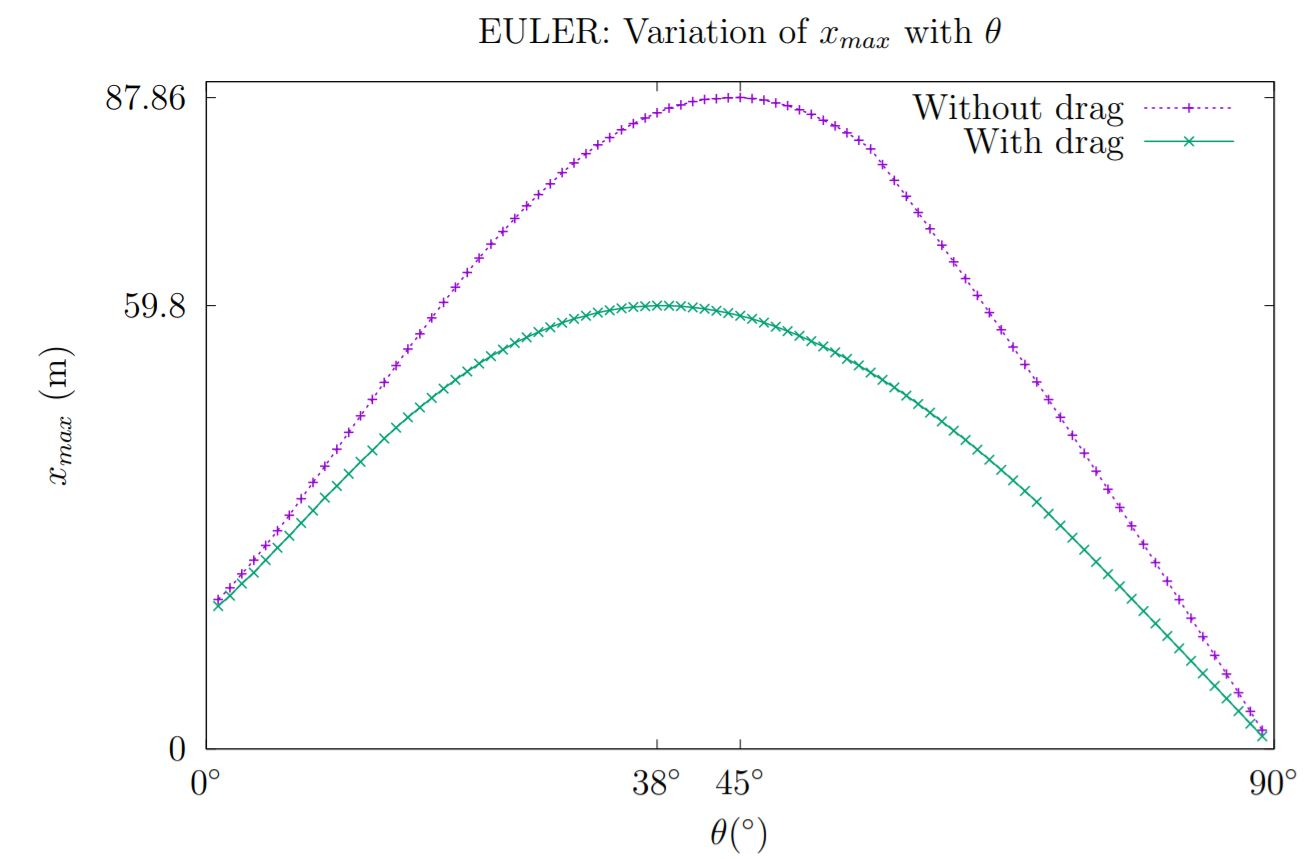
\includegraphics[width=0.85\textwidth]{fig11.JPG}
    \caption{Figure shows the variation of $x_{max}$ with $\theta$, computed using the Euler method}
    \label{fig:fig11.JPEG}
\end{figure}
\end{frame}
%%%%%%%%%%%%%%%%%%%%%%%%%%%%%%%%%%%%%%
\begin{frame}{Results and Analysis}
    \begin{figure}
    \centering
    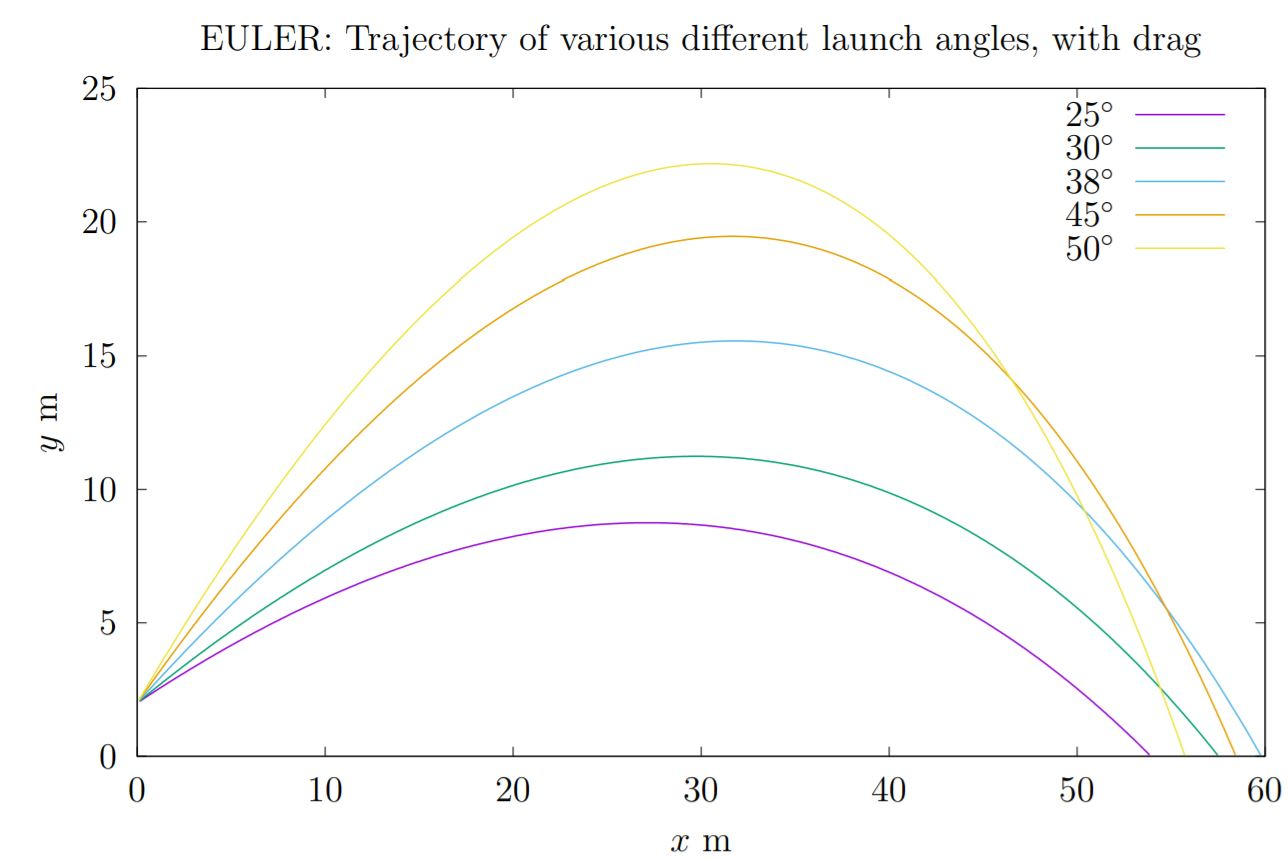
\includegraphics[width=0.85\textwidth]{fig22.JPG}
    \caption{Figure shows trajectories of javelin thrown with different launch angles, computed using the Euler method}
    \label{fig:fig22.JPEG}
\end{figure}
\end{frame}
%%%%%%%%%%%%%%%%%%%%%%%%%%%%%%%%%%%%%%
\begin{frame}{Results and Analysis}
\begin{figure}
    \centering
    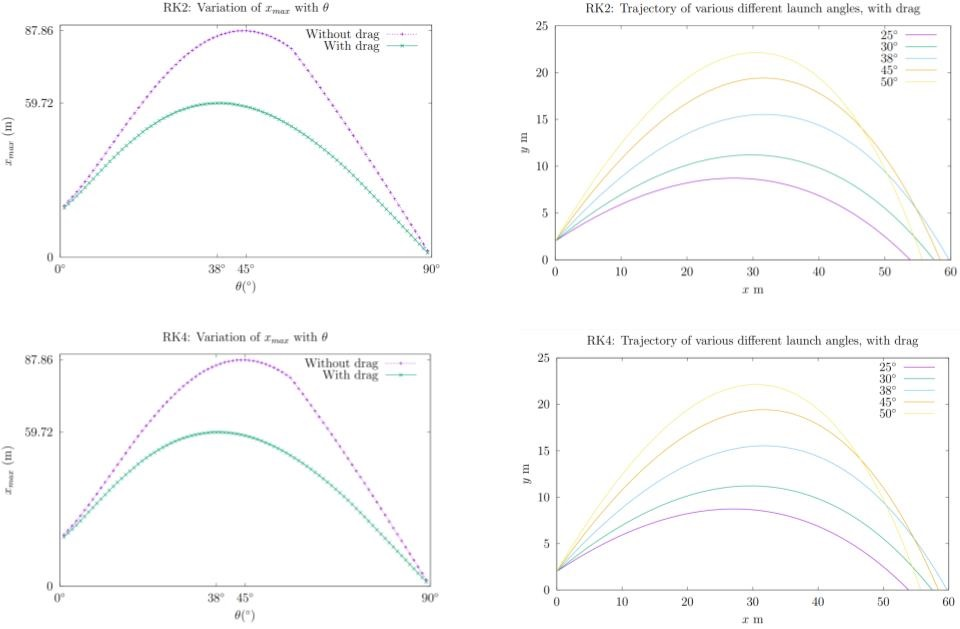
\includegraphics[width=0.99\textwidth]{fig3.JPG}
    \caption{Results with rk2 and rk4 method}
    \label{fig:fig3.JPEG}
\end{figure}
\end{frame}
%%%%%%%%%%%%%%%%%%%%%%%%%%%%%%%%%%%%%%
\begin{frame}[t]{Conclusion}
    \vspace{6.5pt}
    \begin{block}{Primary conclusions}
    \begin{itemize}
        \item Optimal angle = 38$^\circ$, for all cases.
        \item $x_{max}$ = 59.8m by Euler, 59.72m by rk2, rk4. 
        \item Variation in $x_{max}$ for 35$^\circ$ to 40$^\circ$ = 0.23\%, by euler method.
        \item $\therefore$ it depends more on the athlete's execution.
    \end{itemize}
    \end{block}
\end{frame}
%%%%%%%%%%%%%%%%%%%%%%%%%%%%%%%%%%%%%%
\begin{frame}[t]{Learning}
\vspace{6.5pt}
    \begin{block}{Things that we learned:}
        \begin{itemize}
            \item \LaTeX\, (Writing reports, and making beamers)
            \item GNU plot
            \item Euler, rk2, and rk4 methods
            \item Accounting for air drag
            \item Working in a team for an extended period of time
        \end{itemize}
    \end{block}
\end{frame}
\end{document}